%----------------------------------------------------------------------------------------
%	PACKAGES AND THEMES
%----------------------------------------------------------------------------------------

\documentclass{beamer}

\mode<presentation> {

% The Beamer class comes with a number of default slide themes
% which change the colors and layouts of slides. Below this is a list
% of all the themes, uncomment each in turn to see what they look like.

%\usetheme{default}
%\usetheme{AnnArbor}
%\usetheme{Antibes}
%\usetheme{Bergen}
%\usetheme{Berkeley}
%\usetheme{Berlin}
%\usetheme{Boadilla}
%\usetheme{CambridgeUS}
%\usetheme{Copenhagen}
%\usetheme{Darmstadt}
%\usetheme{Dresden}
%\usetheme{Frankfurt}
%\usetheme{Goettingen}
%\usetheme{Hannover}
%\usetheme{Ilmenau}
%\usetheme{JuanLesPins}
%\usetheme{Luebeck}
%\usetheme{Madrid}
%\usetheme{Malmoe}
%\usetheme{Marburg}
%\usetheme{Montpellier}
%\usetheme{PaloAlto}
%\usetheme{Pittsburgh}
%\usetheme{Rochester}
%\usetheme{Singapore}
%\usetheme{Szeged}
%\usetheme{Warsaw}

% As well as themes, the Beamer class has a number of color themes
% for any slide theme. Uncomment each of these in turn to see how it
% changes the colors of your current slide theme.

%\usecolortheme{albatross}
%\usecolortheme{beaver}
%\usecolortheme{beetle}
%\usecolortheme{crane}
%\usecolortheme{dolphin}
%\usecolortheme{dove}
%\usecolortheme{fly}
%\usecolortheme{lily}
%\usecolortheme{orchid}
%\usecolortheme{rose}
%\usecolortheme{seagull}
%\usecolortheme{seahorse}
%\usecolortheme{whale}
%\usecolortheme{wolverine}

%\setbeamertemplate{footline} % To remove the footer line in all slides uncomment this line
%\setbeamertemplate{footline}[page number] % To replace the footer line in all slides with a simple slide count uncomment this line

%\setbeamertemplate{navigation symbols}{} % To remove the navigation symbols from the bottom of all slides uncomment this line
}

\usepackage[utf8]{inputenc}
\usepackage{graphicx} % Allows including images
\usepackage{booktabs} % Allows the use of \toprule, \midrule and \bottomrule in tables
\usepackage{listings}
\usepackage{lmodern} 

\setbeamertemplate{footline}[frame number] 
\setbeamertemplate{footline}{%
  \raisebox{5pt}{\makebox[\paperwidth]{\hfill\makebox[10pt]{\scriptsize\insertframenumber\hspace{5pt}}}}}
\beamertemplatenavigationsymbolsempty


%%%%%%%%%%%%%%%%%%%%%%%%%%%%%%%%%%%%%%%%%
%   TITLE PAGE                          %
%%%%%%%%%%%%%%%%%%%%%%%%%%%%%%%%%%%%%%%%%


\title{Projet Nachos}
\subtitle{M1 Informatique/MOSIG}   
\author{Amine Aït-Mouloud
\\ Sébastien Avril
\\ Jean-Yves Bottraud
\\ El Hadji Malick Diagne
}
\date{Janvier 2015} 
%%%%%%%%%%%%%%%%%%%%%%%%%%%%%%%%%%%%%%%%%

\begin{document}
\frame{ \begin{center}
			
\includegraphics[width=5cm]{LOGO_IM2AG_UJF.eps}
		\end{center}
		\titlepage} 

\begin{frame}{Plan}
    \tableofcontents
\end{frame}

\section{Introduction}
\begin{frame}{Principales fonctionnalités}
	\begin{itemize}
       \item Gestion d'entrées/sorties
       \item Multithreading
       \item Mémoire virtuelle et multi-processus
       \item Système de fichiers
       \item Transmission de données et de fichiers sur le réseau
   \end{itemize}
\end{frame}

\section{Implémentation}
\begin{frame}{Plan}
    \tableofcontents[currentsection]
\end{frame}

\subsection{Console}
\begin{frame}{Console: Lecture/Écriture}
   \begin{itemize}
       \item Pas de choix d'implémentation particulier.
       \item Écriture et lecture bloqués par deux sémaphores différents.
       \item Problème de deux consoles s’exécutant en même temps.
   \end{itemize}
\end{frame}

\subsection{Multithreading}
\begin{frame}{Multithreading: Identifiant et emplacement en pile}
	\begin{center}
    	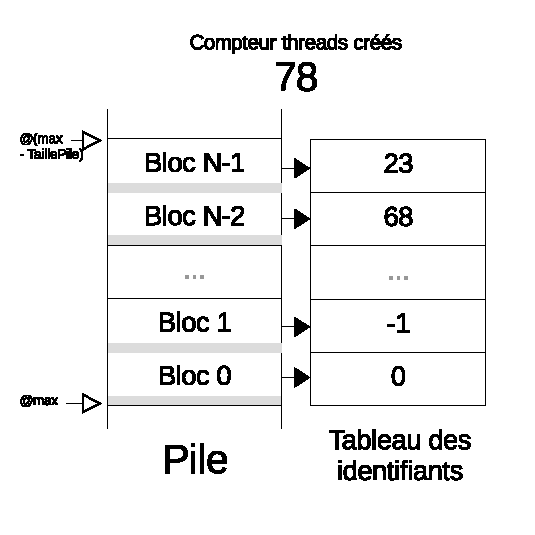
\includegraphics[width=7cm]{../rapport/schema_threads_id.eps}
	\end{center}
   \begin{itemize}
       \item Identifiant unique dans le processus.
   \end{itemize}
\end{frame}

\begin{frame}{Multithreading: Attente}
   \begin{itemize}
       \item Liste de threads en attente et qui ils attendent.
		\item Thread qui attend mis en pause et relancé à la fin du thread qu'il attend.
       \item Attendre si thread en cours d'exécution, retour direct sinon.
       \item Utilisation d'un compteur de thread créés et du tableau des identifiants pour connaître l'état d'exécution d'un thread.
   \end{itemize}
\end{frame}


\subsection{Gestion de la mémoire}
\begin{frame}{Gestion de la mémoire: Multi-processus}
    \begin{itemize}
        \item Partage de la mémoire physique entre différents processus.
        \item Table de pages: mapping entre pages virtuelles du processus et pages physiques.
        \item Utilisation d'un FrameProvider pour obtenir les pages libres.
    \end{itemize}
\end{frame}

\begin{frame}{Gestion de la mémoire: Mapping VPN-PPN}
	\begin{itemize}
		\item METTRE SCHEMA ICI. (Séb?)
    \end{itemize}
\end{frame}

\subsection{Système de fichiers}
\begin{frame}{Système de fichiers}
    \begin{itemize}
		\item 8 fichiers/dossiers maximum par dossier (+ "\texttt{.}" et "\texttt{..}").
		\item Dossier "\texttt{/System}" contient tous les exécutables (à l'image de \texttt{/usr/bin} pour Linux).
    \end{itemize}
\end{frame}

\subsection{Réseau}

\begin{frame}{Réseau: Protocole utilisé}
        \begin{center}
			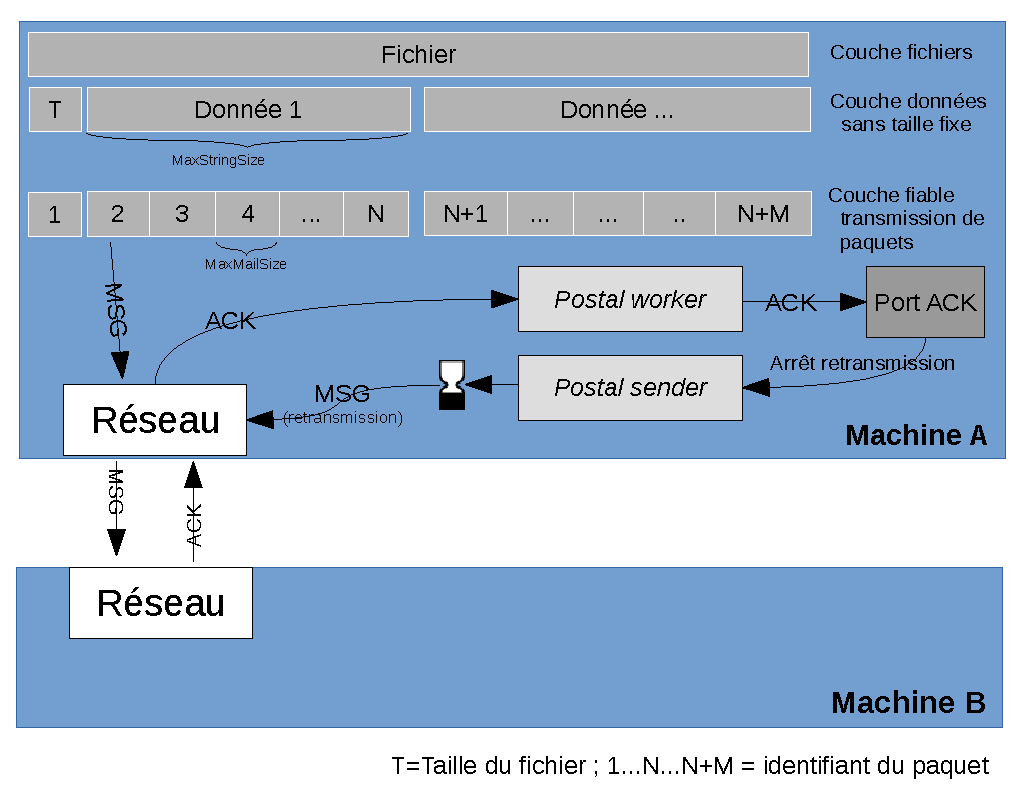
\includegraphics[width=10cm]{schema_reseau.pdf}
		\end{center}
\end{frame}

\begin{frame}{Réseau: API fournie}
    \begin{itemize}
        \item Envoi et réception de données fiable sans limite de taille.
        \item Envoi et réception de fichiers.
    \end{itemize}
\end{frame}

\subsection{Améliorations possibles}
\begin{frame}{Améliorations possibles}
    \begin{itemize}
        \item threads
        	\subitem
        \item mémoire virtuel
        \item système de fichier
        	\subitem table des fichiers ouvert
        \item réseaux
        	\subitem 
    \end{itemize}
\end{frame}

\section{Gestion du projet}
\begin{frame}{Plan}
    \tableofcontents[currentsection]
\end{frame}

\begin{frame}{Gestion du projet}
    \begin{itemize}
        \item repository git
        \item planning
    \end{itemize}
\end{frame}

\section{Conclusion}
\begin{frame}{Plan}
    \tableofcontents[currentsection]
\end{frame}

\subsection{commentaire}
\begin{frame}{commentaire}
	\begin{itemize}
		\item ce qu'on aurait aimé faire
			\subitem scheduler
		\item remarque
	\end{itemize}
\end{frame}

\subsection{conclusion}
\begin{frame}{Conclusion}
    \center{Fin.}
\end{frame}

\end{document}
